%!TEX TS-program = xelatex
\documentclass{beamer}

\usepackage{HSE-theme/beamerthemeHSE} % Подгружаем тему

%%% Работа с русским языком и шрифтами
\usepackage[english,russian]{babel}   % загружает пакет многоязыковой вёрстки
\usepackage{fontspec}      % подготавливает загрузку шрифтов Open Type, True Type и др.
\defaultfontfeatures{Ligatures={TeX},Renderer=Basic}  % свойства шрифтов по умолчанию
\setmainfont[Ligatures={TeX,Historic}]{Myriad Pro} %  установите шрифты Myriad Pro или (при невозможности) замените здесь на другой шрифт, который есть в системе — например, Arial
\setsansfont{Myriad Pro}  %  установите шрифты Myriad Pro или (при невозможности) замените здесь на другой шрифт, который есть в системе — например, Arial
\setmonofont{Courier New}
\uselanguage{russian}
\languagepath{russian}
\deftranslation[to=russian]{Theorem}{Теорема}
\deftranslation[to=russian]{Definition}{Определение}
\deftranslation[to=russian]{Definitions}{Определения}
\deftranslation[to=russian]{Corollary}{Следствие}
\deftranslation[to=russian]{Fact}{Факт}
\deftranslation[to=russian]{Example}{Пример}
\deftranslation[to=russian]{Examples}{Примеры}

\usepackage{alltt}
\usepackage{multicol} 		% Несколько колонок
\graphicspath{{images/}}  	% Папка с картинками

%%% Информация об авторе и выступлении
\title[Disambiguation]{Morphological disambiguation} 
%\subtitle{Подзаголовок презентации / Название конференции}
\author[Francis M. Tyers]{Francis M. Tyers\\ \smallskip \scriptsize \url{ftyers@hse.ru}\\\url{https://www.hse.ru/org/persons/209454856}}
\institute[Высшая школа экономики]{Национальный исследовательский университет \\ «Высшая школа экономики» (Москва)}
\date{\today}

\begin{document}	% Начало презентации

\frame[plain]{\titlepage}	% Титульный слайд

\section{Просто слайд с текстом}
\subsection{Просто слайд с текстом}

\begin{frame}{Introduction}

% Orientation
% Tagsets 



\end{frame}

\begin{frame}{Pipeline}

\begin{onlyenv}<1>
\includegraphics[width=\textwidth]{images/pipeline.eps}
\end{onlyenv}
\begin{onlyenv}<2>
\includegraphics[width=\textwidth]{images/pipeline-4.eps}
\end{onlyenv}

\end{frame}

\begin{frame}{Terminology}

% Part-of-speech tagging
% Morphological disambiguation
% Morphological analysis (~parsing)

\textbf{Part-of-speech tagging:}
   \begin{itemize}
     \item Traditional term, based on approach(es) for English, finite-set of 
       tags for all combinations of lexical category and morphology. \\ ~ \\
       \begin{tabular}{llllp{0.32\textwidth}}
         \hline
         \textbf{In:} & This & is & a & test \\
         ~ & This/PRON & is/VERB & a/DET & test/NOUN \\
         \hline
       \end{tabular}
   \end{itemize}
~\\
\textbf{Morphological disambiguation:}
   \begin{itemize}
      \item More cross-linguistically applicable, conception is of disambiguating
        after morphological analysis. \\  ~ \\
       \begin{tabular}{lllll}
         \hline
         \textbf{In:} & This/DET/PRON & is/VERB & a/DET & test/VERB/NOUN \\
         ~ & This/PRON & is/VERB & a/DET & test/NOUN \\
         \hline
       \end{tabular}
   \end{itemize}  

\end{frame}

\begin{frame}{What is a tagset?}

\end{frame}

\begin{frame}{Example tagsets}

%Penn Treebank style:
%Positional style:
%Universal Dependencies:
  
\begin{onlyenv}<1>
\begin{center}
\textbf{Penn Treebank} 
\end{center}
  \begin{columns}
  
    \begin{column}{0.4\textwidth}
    
    \begin{alltt}
       This/DT \\
       tagset/NNS  \\
       contains/VBZ \\
       48/CD \\
       unique/JJ \\
       tags/NNP  \\
       ./.  \\
    \end{alltt}
    
    \end{column}
    
    \begin{column}{0.6\textwidth}
    
    \begin{itemize}
       \item 48 tags 
       \item Tags are atomic
       \item Principles have been applied to other languages (Chinese, Bengali, \ldots)
       \item Extensible ? 
    \end{itemize}
    \end{column}

  \end{columns}
  
\end{onlyenv}

\begin{onlyenv}<2>
  \begin{center}
  \includegraphics[width=0.9\textwidth]{images/penn-tagset.png}
  \end{center}
\end{onlyenv}

\begin{onlyenv}<3>
\begin{center}
\textbf{Positional tags} 
\end{center}

\end{onlyenv}

\begin{onlyenv}<4>
\begin{center}
\textbf{Mnemonic tags} 
\end{center}

\end{onlyenv}

\begin{onlyenv}<5>
\begin{center}
\textbf{Feature/value pairs} 
\end{center}

\end{onlyenv}

\end{frame}

% Tagset considerations morph<-->syntax

\begin{frame}{Tagset design}

% Ambiguity
% 
% Morphological complexity % Language complexity tagging eng vs. chukchi

\end{frame}

\begin{frame}{Scale of the problem}
% scale of the problem (how many words are ambiguous?) types/tokens

\end{frame}

\begin{frame}{Types of ambiguity}
% Morphological ambiguity ... types

\end{frame}

\begin{frame}{A baseline}
% most freq. class baseline

\end{frame}

% what POS tagging is not... tokenisation/multiwords

% Applications


\begin{frame}{Approaches}
% Approaches

\begin{itemize}
   \item \textbf{Rule-based}:
   \item \textbf{HMM-based}:
   \item \textbf{Averaged perceptron}:
\end{itemize}

\end{frame}

%%%%%%%%%%%%%%%%%%%%%%%%%%%%%%%%%%%%%%%%%%%%%%%%%%%%%%%%%%%%%%%%%%%%%%%%%%%%%%%
%% Rule-based ... CG, ...
\begin{frame}
\centering
{\LARGE {\bf Rule-based } }
\end{frame}

\begin{frame}{History}

\end{frame}

\begin{frame}{Constraint Grammar}

\end{frame}

\begin{frame}{Effort}

\end{frame}

\begin{frame}{Worked example}

\end{frame}

\begin{frame}{Examples}

\end{frame}

%% Rule-application

%%%%%%%%%%%%%%%%%%%%%%%%%%%%%%%%%%%%%%%%%%%%%%%%%%%%%%%%%%%%%%%%%%%%%%%%%%%%%%%
% HMM
\begin{frame}
\centering
{\LARGE {\bf HMM-based } }
\end{frame}

% generative model
\begin{frame}

\end{frame}

% assumptions

% bigrams

% worked example



% extensions

% trigram, other features

% downsides


%%%%%%%%%%%%%%%%%%%%%%%%%%%%%%%%%%%%%%%%%%%%%%%%%%%%%%%%%%%%%%%%%%%%%%%%%%%%%%%
% Averaged Perceptron
\begin{frame}
\centering
{\LARGE {\bf Averaged perceptron} }
\end{frame}

\begin{frame}
% discriminative model

\end{frame}


%%%%%%%%%%%%%%%%%%%%%%%%%%%%%%%%%%%%%%%%%%%%%%%%%%%%%%%%%%%%%%%%%%%%%%%%%%%%%%%

% How much data ?

\begin{frame}{How much data ?}

\end{frame}

\begin{frame}{Time comparison}

% annotation time vs. rule-writing time

% Huldén 20 hours / 148 rules / 113 generic, 35 for wordforms [working from a devel. corpus]
% Tyers 1 month / 299 rules [working from nothing]

% 8000--10000 tokens/month = ~50-60 tokens/hour

\end{frame}

% Combination/voting

\begin{frame}{Tagger combination}



\end{frame}


\begin{frame}{Some taggers}
% some state of the art systems

% specifically for russian:
% pymorphy

% trainable:
% hunpos
% udpipe
% marmot


\end{frame}

\begin{frame}{Practicals}

\begin{itemize}
  \item \textbf{Tagger comparison}:
  \begin{itemize}
     \item Compare five taggers on a language of your choice
  \end{itemize}
  \item \textbf{Constraint grammar}: 
  \begin{itemize}
     \item Select a small text (500 tokens) in a language of your choice
     \item Analyse it with a morphological analyser
     \item Resolve as much of the ambiguity as you can
  \end{itemize}
  \item \textbf{Perceptron tagger}:
  \begin{itemize}
     \item Download \url{https://github.com/ftyers/conllu-perceptron-tagger}
     \item Run it on a language from Universal Dependencies
     \item Improve it so that you get better performance
     \begin{itemize}
       \item Add support for morphological features
       \item Try tweaking other features
     \end{itemize}
  \end{itemize}
\end{itemize}

\end{frame}

\end{document}
